\documentclass{beamer}

% Theme
\usepackage[T1]{fontenc}
\usepackage[default]{gillius}
\usetheme{sintef}

% Math
\usepackage{amsfonts,amsmath,oldgerm}
\usepackage{mathtools}
\usepackage{lmodern}
\usefonttheme[onlymath]{serif}
\newcommand\norm[1]{\lVert#1\rVert}
\DeclareMathAlphabet{\mathsc}{T1}{lmr}{m}{sc}

% Code
\usepackage{algpseudocode}

% Figures
\usepackage{graphicx}
\usepackage{caption}
\usepackage{subcaption}

% Tables
\usepackage{array}
\usepackage{tabularx}
\usepackage{colortbl}

% Boxes
\usepackage{xcolor}
\usepackage{tcolorbox}
\usepackage{adjustbox}
\tcbuselibrary{skins}
\tcbset{tab2/.style={enhanced,fonttitle=\bfseries,fontupper=\small\sffamily,
colback=yellow!10!white,colframe=red!50!black,colbacktitle=Salmon!40!white,
coltitle=black,center title}}

% Shapes
\usepackage{tikz}
\usetikzlibrary{shapes,arrows, positioning, calc}  
\newcommand{\greenplus}[0]{\begin{tikzpicture}
    \draw[green, line width=5pt] (-0.01,0) -- (0.01,0);
    \draw[green, line width=5pt] (0,-0.01) -- (0,0.01);
    \node[minimum width=0.2cm] at (current bounding box.east) {};
\end{tikzpicture}}
\newcommand{\redminus}[0]{\begin{tikzpicture}
    \draw[red, line width=5pt] (0,-0.01) -- (0,0.01);
    \node[minimum width=0.2cm] at (current bounding box.east) {};
\end{tikzpicture}}

% Random commands
\newcolumntype{Y}{>{\raggedleft\arraybackslash}X}
\newcommand{\hrefcol}[2]{\textcolor{cyan}{\href{#1}{#2}}}
\newcommand{\testcolor}[1]{\colorbox{#1}{\textcolor{#1}{test}}~\texttt{#1}}
\newcommand*{\defeq}{\stackrel{\text{def}}{=}}  % https://latex.org/forum/viewtopic.php?t=15406
\newcommand*{\textfluent}[1]{\textsc{#1}}
% comandi per le parole più comuni
\newcommand*{\sck}{\textfluent{K}}
\newcommand*{\knows}{\textbf{Knows}}
\newcommand*{\scdo}{\textfluent{do}}
\newcommand*{\scsense}{\textfluent{sense}}
\newcommand*{\scread}{\textfluent{read}}
\newcommand*{\scdrop}{\textfluent{drop}}
\newcommand*{\scposs}{\textfluent{Poss}}
\newcommand*{\scp}{\textfluent{P}}
\newcommand*{\scq}{\textfluent{Q}}
\newcommand*{\scsr}{\textfluent{sr}}
\newcommand*{\scyes}{``\textfluent{yes}"} % solo in math mode
\newcommand*{\scno}{``\textfluent{no}"}   % solo in math mode
\newcommand*{\scok}{``\textfluent{ok}"}   % solo in math mode

\titlebackground*{assets/background}

\title{Knowledge, action, and the frame problem}
\course{Reasoning about Actions}
\author{Francesco Petri, Charlotte Primiceri and Flavio Maiorana}
\date{\today}

\begin{document}
\maketitle

% \section{}
% \begin{frame}{Introduction}
% \end{frame}

\footlinecolor{sintefyellow}
\section{Scherl and Levesque's Approach}
%!TEX root = presentation.tex

% memo: mille modi per centrare
% https://tex.stackexchange.com/questions/449578/basic-how-can-i-stop-centering-a-text

\subsection{Introduction}

\begin{frame}{Outline}
    Situation calculus provides a framework for reasoning about actions.

    This work presents an expansion to handle the \textit{knowledge} possessed or acquired by the agent,
    and allow it to shape the agent's decisions.
    \begin{itemize}%[<+->]
        \item Knowledge is represented by one additional fluent
        \item Uniform axiomatization with the rest of sitcalc
        \item Ordinary actions and knowledge-producing ones are strictly separated
        \item Easy expansion of regression as defined in [Reiter2001]
        \item Desirable properties are direct consequences of the axiomatization \\
                (e.g. knowledge persistence / memory)
    \end{itemize}
\end{frame}

% opzionale
\begin{frame}{...}
    Opzionale

    Un paio di azioni ordinarie e un paio di azioni di conoscenza di esempio, giusto per inquadrare il discorso
\end{frame}

\subsection{Knowledge as a fluent}

\begin{frame}[fragile]{The K fluent}
    \huge
    \[ \sck(s', s) \]
    \normalsize

    Defines an accessibility relation between situations.

    % Informal definition: \( \sck(s', s) \) is true if, given its current knowledge,
    % the situations \(s\) and \(s'\) are indistinguishable to the agent.

    \begin{block}{(Informal) definition}
        \( \sck(s',s) \) is true if an agent in situation \(s\)
        could mistake the current situation for the other \(s'\),
        given its current knowledge.
    \end{block}
\end{frame}

\begin{frame}{Knowledge}
    \begin{block}{Definition of knowledge}
        A fluent is known to be true (false) in a situation \(s\)
        if and only if it is true (false)
        in all situations accessible from \(s\).
    \end{block}

    Shorthand notation: \( \knows(\phi, s) \defeq \forall s' \: \sck(s',s) \rightarrow \phi(s') \)
\end{frame}

\begin{frame}{Knowledge-producing actions}
    Actions that have an effect on the agent's knowledge

    \begin{block}{SENSE actions}
        % Learn whether a fluent is true or false. Example: check if a door is open or closed.
        Learn the truth value of a formula. Example: check if a door is open or closed.
        \[
            \knows(\textfluent{P}, \scdo(\scsense_\text{P}, s))
            \lor
            \knows(\lnot \textfluent{P}, \scdo(\scsense_\text{P}, s))
        \]
    \end{block}

    \begin{block}{READ actions}
        % Learn what a functional term refers to. Example: read a number on a sheet of paper.
        Learn the value of a term. Example: read a number on a sheet of paper.
        \[
            \exists x \: \knows(\tau = x, \scdo(\scread_\tau, s))
        \]
    \end{block}

    \emph{Assumption: ordinary and knowledge-producing actions are strictly separated.}
\end{frame}

\subsection{Defining a successor state axiom for K}

\begin{frame}{Knowledge effects}
    In order to complete the specification of the \sck fluent,
    we need to define its successor state axiom,
    determining how ordinary actions and knowledge-producing actions affect it.

    Consider this case study with three accessible situations. The agent is in S1.

    \begin{center}
        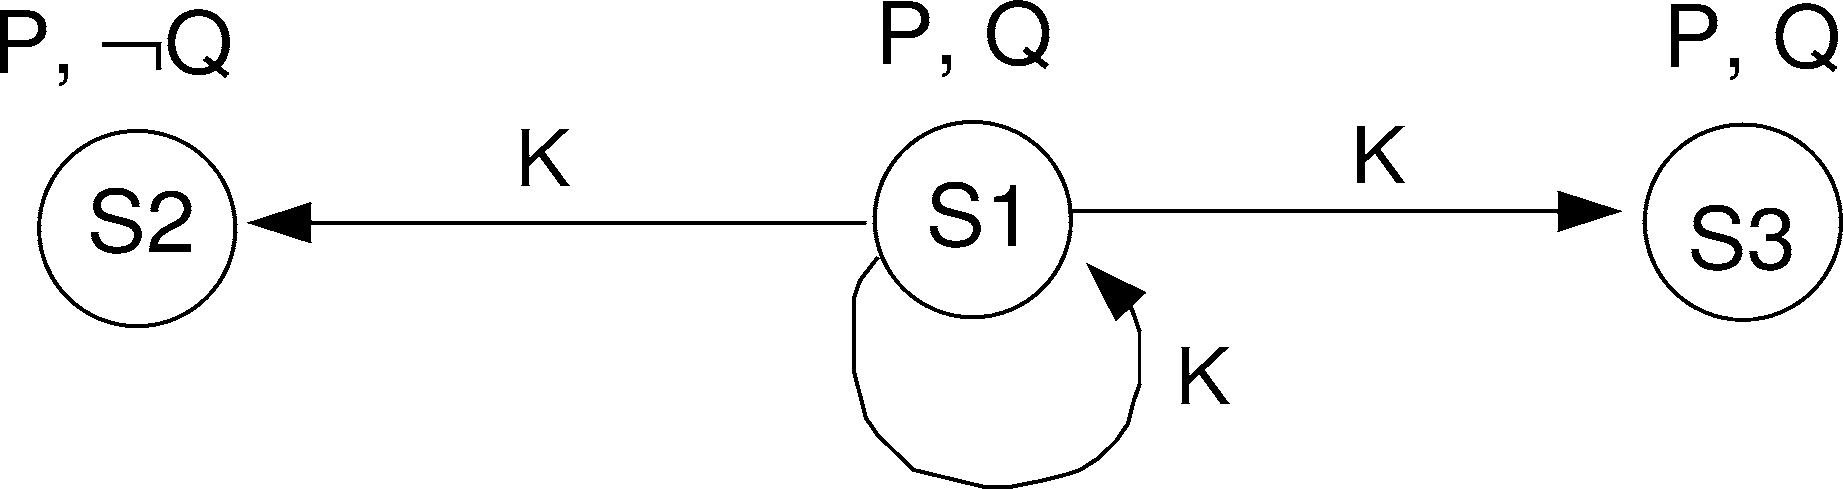
\includegraphics[width=0.6\textwidth]{assets/3states_noactions.png}
    \end{center}

    \[ \knows(\textfluent{P}, S1) \land \lnot \knows(\textfluent{Q}, S1) \]
\end{frame}

\begin{frame}{Ordinary actions}
    Assume the agent performs a \textfluent{drop} action.

    \begin{block}{Informal idea}
        The agent cannot distinguish the current situation \(s\) from all the other
        \(s'\) accessible from it. Therefore, after executing the action,
        the agent may believe to be in any situation resulting from any \(s'\) after executing \textfluent{drop}.
    \end{block}

    \begin{block}{Axiomatization}
        \[ \sck(s'', \scdo(\scdrop, s)) \equiv \exists s' \: (\scposs(\scdrop, s') \land \sck(s',s) \land s'' = \scdo(\scdrop, s')) \]
    \end{block}
\end{frame}

\begin{frame}{Ordinary actions}
    Pippo
\end{frame}

\begin{frame}{Knowledge-producing actions}
    Pippo
\end{frame}

\begin{frame}{The successor state axiom for K}
    Pippo
\end{frame}

\begin{frame}{<varie ed eventuali>}
    Pippo
\end{frame}


\footlinecolor{sinteflilla}
\section{Regression}

\footlinecolor{sintefdarkgreen}
\section{Example: The Gardening Robot}

\begin{frame}{The Problem}
    \vspace*{-0.5cm}
    \begin{itemize}
        \item A robot has to manage \textbf{n plants} in a garden.
        \item The robot performs an action on one plant at a time.
        \item \textbf{A plant can be watered only if it is dry and the temperature is known.}
        \item The robot has access to a watering can with unlimited capacity.
        \item The robot performs action on an object only if it is near it.
        \item The robot can hold only one object at a time.
    \end{itemize}
\end{frame}

\subsection{Axiomatization}

\begin{frame}[fragile]{(Non)Fluents}
    \vspace*{-0.5cm}
    \begin{block}{Fluents}
        \begin{itemize}
            \item $\textsc{Near}(x,s) \rightarrow$ Robot is near object x in situation s
            \item $\textsc{Holding}(x,s) \rightarrow$ Robot is holding object x in situation s
            \item $\textsc{Moist}(p,s) \rightarrow$ Plant p is moist in situation s
            \item $\textsc{Temperature}(p,s) \rightarrow$ Temperature value of the spot near plant p
            \item $\textsc{MoistPlants}(s) \rightarrow$ Number of moist plants
        \end{itemize}
    \end{block}
    \begin{block}{Non-Fluents}
        \begin{itemize}
            \item $\textsc{WateringCan}(x) \rightarrow $ Object x is a watering can
            \item $\textsc{Thermometer}(x) \rightarrow $ Object x is a thermometer
            \item $\textsc{Moisturemeter}(x) \rightarrow $ Object x is a moisturemeter
        \end{itemize}
    \end{block}
\end{frame}

% The policy ensures a sharp division between knowledge-producing actions and ordinary
% actions. Without this policy there is nothing to prevent us from having an action such as
% open the bag which causes the bag to be open and makes the agent aware of the content of
% the bag.
\begin{frame}{Actions}
    \vspace*{-0.5cm}
    All actions are to be axiomatized as affecting only either the K fluent or other fluents.
    \begin{block}{Normal}
        \begin{itemize}
            \item $\textsc{goto}(x) \rightarrow$ Go to object x
            \item $\textsc{water}(p) \rightarrow$ Water plant p
            \item $\textsc{pickup}(x) \rightarrow$ Pick up object x
            \item $\textsc{putdown}(x) \rightarrow$ Put down object x
        \end{itemize}
    \end{block}
    \begin{block}{Knowledge}
        \begin{itemize}
            \item $\textsc{checkmoisture}(p) \rightarrow$ Check moisture of plant p
            \item $\textsc{checktemperature}(p) \rightarrow$ Check the temperature of the spot near plant p
        \end{itemize}
    \end{block}
\end{frame}

\begin{frame}{Effects}
    \vspace*{-0.5cm}
    \begin{block}{Sensing Result Axioms}
        \begin{itemize}
            \item $\textsc{sr}(\textsc{goto}(x),s) = r\equiv r = \scok$
            \item $\textsc{sr}(\textsc{checkmoisture}(p),s) = r \equiv (r = \scyes \land \textsc{Moist}(p,s)) \lor (r = \scno \land \neg \textsc{Moist}(p,s))$
            % It specifies that after doing the checkmoisture(p) action, the agent knows whether or not p is moist.
            \item $\textsc{sr}(\textsc{checktemperature}(p),s) = r \equiv r = \textsc{Temperature}(p,s)$
        \end{itemize}
    \end{block}
    \begin{block}{Knowledge Action Effects}
        \begin{itemize}
            \item \textbf{Kwhether}$(\textsc{Moist}(p), \textsc{do}(\textsc{checkmoisture}(p),s))$
            \item \textbf{Kref}$(\textsc{Temperature}(p), \textsc{do}(\textsc{checktemperature}(p),s))$
        \end{itemize}
    \end{block}
\end{frame}

\begin{frame}{Preconditions}
    \begin{itemize}
        \item $\textsc{Poss}\left( \textsc{water}(p), s \right) \equiv \textsc{Near}(p,s) \land \textsc{Holding}(x,s) \land \textsc{WateringCan}(x) \land$ \textbf{Knows}$(\neg\textsc{Moist}(p),s) \land $ \textbf{Kref}$(\textsc{Temperature}(p),s)$
        \item $\textsc{Poss}\left( \textsc{pickup}(x), s \right) \equiv \textsc{Near}(x,s) \land \neg \exists y.\textsc{Holding}(y,s)$
        \item $\textsc{Poss}\left( \textsc{putdown}(x), s \right) \equiv \textsc{Holding}(x,s)$
        \item $\textsc{Poss}\left( \textsc{checkmoisture}(p), s \right) \equiv \textsc{Near}(p,s) \land \textsc{Holding}(x,s) \land \textsc{Moisturemeter}(x)$
        \item $\textsc{Poss}\left( \textsc{checktemperature}(p), s \right) \equiv \textsc{Near}(p,s) \land \textsc{Holding}(x,s) \land \textsc{Thermometer}(x)$
    \end{itemize}
\end{frame}

\begin{frame}{Successor State Axioms}
    In general $F(x,\textsc{do}(\alpha,s)) \equiv \Phi_F^+(x,a,s) \lor (F(x,s) \land \neg \Phi_F^-(x,a,s))$
    \vspace*{0.5cm}
    \begin{itemize}
        \item $\textsc{Near}(x,\textsc{do}(\alpha,s)) \equiv \alpha = \textsc{goto}(x)
        \lor \left( \textsc{Near}(x,s) \land \neg \exists
        y.\alpha=\textsc{goto}(y)\right)$
        \item $\textsc{Holding}(x,\textsc{do}(\alpha,s))\equiv \alpha = \textsc{pickup}(x) \lor \left( Holding(x,s) \land \neg \exists r.\alpha=\textsc{putdown}(x)\right)$
        \item $\textsc{Moist}(p,\textsc{do}(\alpha,s)) \equiv \alpha = \textsc{water}(p) \lor \left( \textsc{Moist}(p,s) \land \neg \exists r.\alpha = \textsc{water}(p) \right)$ 
        \item $\textsc{Temperature}(p,\textsc{do}(\alpha,s)) \equiv \textsc{Temperature}(p,s)$ 
        \item $\textsc{MoistPlants}(p,\textsc{do}(\alpha,s)) = n \equiv \left( \textsc{MoistPlants}(p,s) = n-1 \land \alpha = \textsc{water}(p) \right) 
        \lor \left( \textsc{MoistPlants}(p,s) = n\right)$
    \end{itemize}
\end{frame}

\begin{frame}{Theorems}
    \begin{enumerate}
        \item Knowledge-producing actions do not change the state of the world. If $\scp(s)$ then $\scp(\scdo(\alpha, s))$, given that $\alpha$ is knowledge-producing and $\scp$ is not $\sck$
        \item Nothing is learned about $\scp$ by doing action $\alpha$, as long as $\alpha$ does not affect $\scp$.
        \item Agents know the consequences of knowledge acquired through knowledge-producing actions.
        \item If the agent knows $\scp$ at $s$, then $\scp$ is also known at $\scdo (\alpha,s)$ as long as the effect of $\alpha$ is not to make $\scp$ false.
        \item Agents know the effects of (ordinary) actions.
    \end{enumerate}
\end{frame}

\subsection{Instantiation}

\begin{frame}[fragile]{Initial Situation}
    \begin{itemize}
        \item $\textsc{WateringCan}(c)$
        \item $\textsc{Thermometer}(t)$
        \item $\textsc{Moisturemeter}(m)$
        \item $\textsc{Plant}(p_1)$ \\
        \hspace{0.5cm}\vdots
        \item $\textsc{Plant}(p_n)$
        \item $\textsc{Near}(c)$
    \end{itemize}
    \begin{block}{Goal}
        Have $n$ moist plants, namely $\textsc{MoistPlants}(p,s) = n$
    \end{block}
\end{frame}

\begin{frame}{Solution}
    \vspace*{-1cm}
    For every plant $p$, with the following situations
    \hspace*{-1cm}
    \centering
    \begin{minipage}{0.8\linewidth}
        \vspace{5pt}
        $\textsc{S}_1 = \\ \textsc{do}(\textsc{putdown}(m),\textsc{do}(\textsc{checkmoisture}(p), \\\textsc{do}(\textsc{goto}(p),\textsc{do}(\textsc{pickup}(m),\textsc{do}(\textsc{goto}(m),\textsc{S}_0)))))$ \\
        $\textsc{S}_2 = \\ \textsc{do}(\textsc{putdown}(t),\textsc{do}(\textsc{checktemperature}(p), \\\textsc{do}(\textsc{pickup}(t),\textsc{do}(\textsc{goto}(t),\textsc{S}_1))))$ \\
        $\textsc{S}_3 = \\ \textsc{do}(\textsc{putdown}(c),\textsc{do}(\textsc{water}(p), \\\textsc{do}(\textsc{pickup}(c),\textsc{do}(\textsc{goto}(c),\textsc{S}_2))))$
    \end{minipage} \\
    \vspace{15pt}
    In the end, we need to entail that $\textsc{MoistPlants}(p, s) = n$ \\
    We can use the successor state axioms for that
\end{frame}

\begin{frame}{Legality testing (with a different $S_0$)}
    \centering
    $\textsc{do}(\textsc{water}(p), \textsc{do}(\textsc{pickup}(c),\textsc{do}(\textsc{goto}(c),\textsc{do}(\textsc{putdown}(t),\textsc{S}_0))))$ \\
    $\Downarrow$ \\
    We need to entail \\$\textsc{Near}(p,\textsc{S}_0) \land \textsc{Holding}(t,\textsc{S}_0) \land 
    \textsc{Thermometer}(t,\textsc{S}_0) \land$ \textbf{Knows}$(\neg \textsc{Moist}(p,\textsc{S}_0)) \land$ \textbf{Kref}$(\textsc{Temperature}(p),\textsc{do}(\textsc{checktemperature}(p),\textsc{S}_0))$ \\
    $\Downarrow$ \\
    $\exists y.y = \textsc{Temperature}(p,s)$
\end{frame}

\begin{frame}[fragile]{Golog}
    \vspace*{-1.5cm}
    \hspace*{2.5cm}
    \begin{minipage}{\linewidth}
        \begin{algorithmic}[1]
            \While{$\neg \mathbf{Knows}(\textsc{HealthyPlants} = n)$} \\
            \quad ($\mathit{\Pi}$p) \textsc{goto}(p); \\
            \quad \quad $\textsc{checkmoisture}(p)$; \\
            \quad \quad \textbf{if Knows}$(\neg \textsc{Moist}(p))$ \\
            \quad \quad \quad \textsc{goto}(t); \\
            \quad \quad \quad \quad \textsc{pickup}(t); \\
            \quad \quad \quad \quad \textsc{goto}(p); \\
            \quad \quad \quad \quad $\textsc{checktemperature}(p)$; \\
            \quad \quad \quad \quad \textsc{putdown}(t); \\
            \quad \quad \quad \textsc{goto}(c); \\
            \quad \quad \quad \quad \textsc{pickup}(c); \\
            \quad \quad \quad \quad \textsc{goto}(p); \\
            \quad \quad \quad \quad $\textsc{water}(p)$; \\
            \quad \quad \quad \quad \textsc{putdown}(c);
            \EndWhile
        \end{algorithmic}
    \end{minipage}
\end{frame}

\footlinecolor{}

\backmatter
\end{document}
